\documentclass[11pt,letterpaper]{article}
\usepackage{anysize}
\usepackage{indentfirst}
\usepackage{sectsty}
\usepackage{amsmath}
\usepackage{hyperref}
\usepackage{graphicx}
\usepackage{chngpage}
\usepackage{enumerate}
\hypersetup{
	colorlinks=true, 
	linkcolor=blue, 
	urlcolor=blue, 
	pdfnewwindow=true, 
	citecolor=black
}
\urlstyle{same}
\linespread{1.2}

\begin{document}

\begin{titlepage}
    \vspace*{4cm}
    \begin{flushright}
    {\huge
        Project 3\\[5mm]
    }
    {\large
        CS325 | Spring 2015
     }
    \end{flushright}
\hrule
    \begin{flushright}
	by Group 2\\
	Vedanth Narayanan\\
	Jonathan Merrill\\
	Tracie Lee\\
    \vfill
	\today\\
    \end{flushright}
\end{titlepage}

\raggedright

\section{Transshipment Model}
\subsection*{Part A}


\subsection*{Part B}


\subsection*{Part C}
	

\subsection*{Part D}


\section{Modified from DPV 7.16}
\subsection*{Part A}
\begin{enumerate}
	\item The following is the objective function for this part of the problem. We know this because the question requires us to find the solution with the least number of calories, and the following equation has the necessary values to be able to figure that out. \\
	Note: The variables ($v_1 ... v_8$) correspond to the ingredients mentioned in the problem in order, starting from Tomato to Oil.
	\begin{equation*}
	Minimize (21v_1 + 16v_2 + 40v_3 + 41v_4 + 585v_5 + 120v_6 + 164v_7 + 884v_8)
	\end{equation*}
	The following are all the constraints that the problem mentioned in the beginning.\\
	Protein:
	\begin{equation*}
	(0.85v_1+1.62v_2+2.86v_3+0.93v_4+23.4v_5+16v_6+9v_7) \geq 15
	\end{equation*}
	Fat:
	\begin{equation*}
	8 \geq (0.33v_1+0.2v_2+0.39v_3+0.24v_4+48.7v_5+5v_6+2.6v_7+100v_8) \geq 2
	\end{equation*}
	Carbohydrates:
	\begin{equation*}
	(4.64v_1+2.37v_2+3.63v_3+9.58v_4+15v_5+3v_6+27v_7) \geq 4
	\end{equation*}
	Sodium:
	\begin{equation*}
	(9v_1+28v_2+65v_3+69v_4+3.8v_5+120v_6+78v_7) \leq 200
	\end{equation*}
	Leafy Greens:
	\begin{align*}
	\frac{v_2 + v_3}{v_1 + v_2 + v_3 + v_4 + v_5 + v_6 + v_7 + v_8} \geq \frac{4}{10} \\
	v_2 + v_3 \geq \frac{4}{10} \cdot \left( v_1 + v_2 + v_3 + v_4 + v_5 + v_6 + v_7 + v_8\right) \\
	v_2 + v_3 \geq 0.4(v_1) + 0.4(v_2) + 0.4(v_3) + 0.4(v_4) + 0.4(v_5) + 0.4(v_6) + 0.4(v_7) + 0.4(v_8) \\
	v_2 + v_3 - 0.4(v_1) - 0.4(v_2) - 0.4(v_3) - 0.4(v_4) - 0.4(v_5) - 0.4(v_6) - 0.4(v_7) - 0.4(v_8) \geq &0 \\
	\end{align*}
	In the above equation, counting from the top, I know that $v_2$ and $v_3$ are Lettuce and Spinach. Also, the last equation is a simplified version of the first.
	
	\item LINDO was used for this problem and the following is what we got.
	\begin{verbatim}
MIN 21V1 + 16V2 + 40V3 + 41V4 + 585V5 + 120V6 + 164V7 + 884V8
ST
	0.85V1 + 1.62V2 + 2.86V3 + 0.93V4 + 23.4V5 + 16V6 + 9V7 >= 15
	0.33V1 + 0.2V2 + 0.39V3 + 0.24V4 + 48.7V5 + 5V6 + 2.6V7 + 100V8 >= 2
	0.33V1 + 0.2V2 + 0.39V3 + 0.24V4 + 48.7V5 + 5V6 + 2.6V7 + 100V8 <= 8
	4.64V1 + 2.37V2 + 3.63V3 + 9.58V4 + 15V5 + 3V6 + 27V7 >= 4
	9V1 + 28V2 + 65V3 + 69V4 + 3.8V5 + 120V6 + 78V7 <= 200
	V2 + V3 - 0.4V1 - .4V2 - .4V3 - .4V4 - .4V5 - .4V6 - .4V7 - .4V8 > 0
	V1 >= 0 
	V2 >= 0
	V3 >= 0
	V4 >= 0
	V5 >= 0
	V6 >= 0
	V7 >= 0
	V8 >= 0
END
	\end{verbatim}
	
	The result we got back is the following:
	\begin{verbatim}
 LP OPTIMUM FOUND AT STEP     12
 OBJECTIVE FUNCTION VALUE
 1)      114.7541
 VARIABLE        VALUE          REDUCED COST
 V1         0.000000         16.901640
 V2         0.585480          0.000000
 V3         0.000000         14.513662
 V4         0.000000         36.289616
 V5         0.000000        408.387970
 V6         0.878220          0.000000
 V7         0.000000         97.551910
 V8         0.000000        886.404358
	\end{verbatim}
	\item We take the values we got in the problem and multiply them by the corresponding costs as mentioned in the question. The following is the answer:
	\begin{align*}
	0.58548(0.75) + 0.87822(2.15) = \$2.33
	\end{align*}
\end{enumerate}

\subsection*{Part B}
\begin{enumerate}
	\item The objective function for this equation is the following:
	\begin{align*}
	Minimize(1.00v_1+0.75v_2+0.50v_3+0.50v_4+0.45v_5+2.15v_6+0.95v_7+2.00v_8)
	\end{align*}
	The constraint equations are mostly the same from the previous problem. The only addition is the objective function from Part A. We know that the least calorie is going to be 114.75, so we decided to add a constraint so that the calorie count will be greater than or equal to that value.
	\begin{align*}
	21V1 + 16V2 + 40V3 + 41V4 + 585V5 + 120V6 + 164V7 + 884V8 >= 114.75
	\end{align*}
	
	\item Once again LINDO was used for this problem.
	\begin{verbatim}
MIN 1.00V1 + 0.75V2 + 0.50V3 + 0.50V4 + 0.45V5 + 2.15V6 + 0.95V7 + 2V8
ST
	0.85V1 + 1.62V2 + 2.86V3 + 0.93V4 + 23.4V5 + 16V6 + 9v7 >= 15
	0.33V1 + 0.2V2 + 0.39V3 + 0.24V4 + 48.7V5 + 5V6 + 2.6V7 + 100v8 >= 2
	0.33V1 + 0.2V2 + 0.39V3 + 0.24V4 + 48.7V5 + 5V6 + 2.6V7 + 100V8 <= 8
	4.64V1 + 2.37V2 + 3.63V3 + 9.58V4 + 15V5 + 3V6 + 27V7 >= 4
	9V1 + 28V2 + 65V3 + 69V4 + 3.8V5 + 120V6 + 78V7 <= 200
	V2 + V3 - .4V1 - .4V2 - .4V3 - .4V4 - .4V5 - .4V6 - .4V7 - .4V8 > 0
	21V1 + 16V2 + 40V3 + 41V4 + 585V5 + 120V6 + 164V7 + 884V8 >= 114.75
	V1 >= 0 
	V2 >= 0
	V3 >= 0
	V4 >= 0
	V5 >= 0
	V6 >= 0
	V7 >= 0
	V8 >= 0
END
	\end{verbatim}

	The following is the result.
	\begin{verbatim}
 LP OPTIMUM FOUND AT STEP      0
 OBJECTIVE FUNCTION VALUE
 1)      1.554133
 VARIABLE        VALUE          REDUCED COST
 V1         0.000000          1.002081
 V2         0.000000          0.402912
 V3         0.832298          0.000000
 V4         0.000000          0.486914
 V5         0.096083          0.000000
 V6         0.000000          0.405609
 V7         1.152364          0.000000
 V8         0.000000          7.281258
	\end{verbatim}
	\item Similar to that of Part A, we use the values we got above and apply them to the Energy column in the table that was given to us.
	\begin{align*}
	40(0.832298) + 585(0.096083) + 164(1.152364) = 278.49 calories
	\end{align*} 
\end{enumerate}

\subsection*{Part C}
\begin{enumerate}
	\item It's important to start off by saying that there are always sacrifices to be made. It comes down to priority, and which requirement is more important. This being said, there are a variety of things that Veronica could do to reach her goal. One of the first things to take notice is how both sunflower seeds and oil are really high in calorie. If she wanted to advertise that her salads were less than 250 calories, perhaps looking for an alternative to sunflower seeds and oil may help. If there were ingredients with lesser calories, then the chances of increasing the combinations for the salad are high. \\
	On the other hand, Veronica could buy cheaper ingredients to be able to meet her cost requirement. This also possibly means forgoing her calorie requirement. Another cost saving technique might be trying to use the least number of ingredients. Part A actually happened to do this. With just lettuce and smoked tofu, while the salad seemed slightly boring, it met all the requirements that were set in the problem. On the same idea, perhaps looking for newer ingredients that could do achieve the same effect would be useful too.
	The possible solution maybe involves widening the original requirements that were set. For example, decreasing the protein requirement to 13g, increasing the fat range to 2-10g, 200-220mg of sodium, and 35\% leafy greens by mass. With the widening of ranges, Veronica would get more opportunities to either save money, or decrease the calorie count.
	\item From Part A, I would suggest using calorie effective method. The ingredients involved here are lettuce and smoked tofu. The cost is \$2.33, but the calorie count will be 114.75. 
	\item If she sold these, Veronica would make about \$2.67. This definitely does not meet the expectation she set, but its important to note that the calorie count is far below 250, and she will be selling more of them. What she loses in profit per salad, she will make it up in the amount of salads she sells.\\

	Note: Customer enjoyment is not taken into account in this problem, but if that was taken into account, then it will definitely matter! We do believe that it will make a difference.
\end{enumerate}

\section{Regression Solution via Linear Programming}
\subsection*{Part A}
\textbf{Objective}: min $\sum\limits_{i=1}^n |y_i -  (a_1x_i + a_0)|$\vspace{8pt}

\textbf{Constraint Equations}

\begin{tabular}{l l l}
$a_0+a_1+z_1\geq3$	&  & $a_0+a_1-z_1\leq3$\\
$a_0+a_1+z_2\geq5$ 	& & $a_0+a_1-z_2\leq5$\\
$a_0+2a_1+z_3\geq13$	& & $a_0+2a_1-z_3\leq13$\\
$a_0+3a_1+z_4\geq8$	& & $a_0+3a_1-z_4\leq8$\\
$a_0+4a_1+z_5\geq10$	& & $a_0+4a_1-z_5\leq10$\\
$a_0+5a_1+z_6\geq14$	& & $a_0+5a_1-z_6\leq14$\\
$a_0+6a_1+z_7\geq18$	& & $a_0+6a_1-z_7\leq18$\\
\end{tabular}\vspace{8pt}

%\textbf{LAD equation}: $y = 2.6x + 2.4$\vspace{8pt}

\textbf{Sum of absolute deviations}: 13.8\vspace{8pt}


\centerline{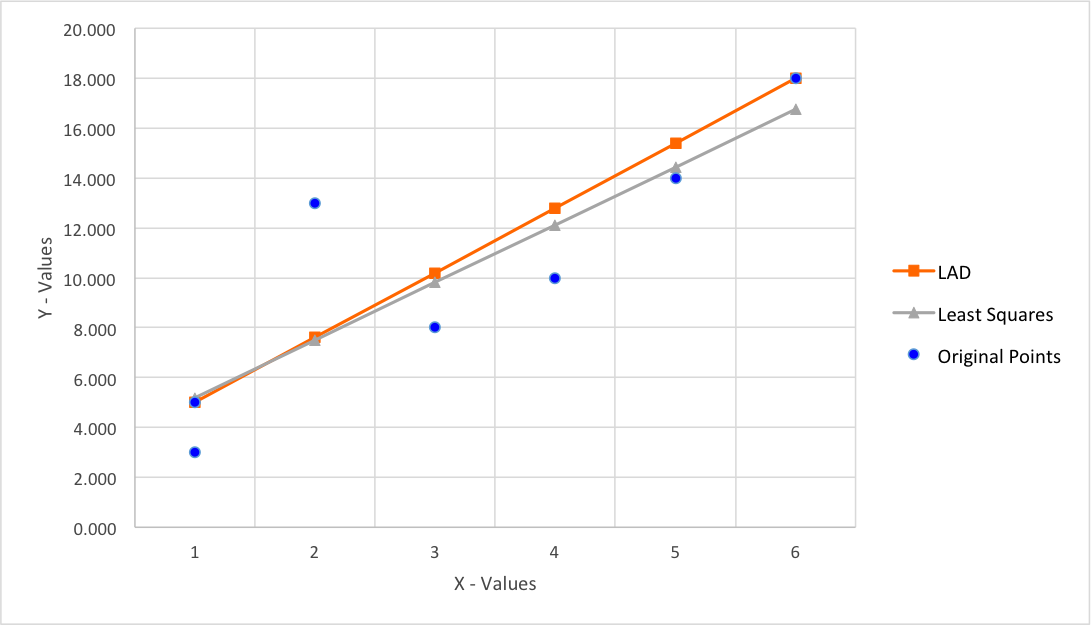
\includegraphics[width=7in]{lad.png}}\vspace{8pt}

This was calculated in Lindo using the constraint equations listed above to obtain the LAD equation $y = 2.6x + 2.4$. In this case, the LAD is close to the original Least Squares solution, especially for x-values close to 0. It appears that as the value of x grows, the gap between the 2 lines will widen.\vspace{8pt}

Lindo code:\vspace{8pt}

\begin{verbatim}
MIN X + Y + Z
ST
    A0+A1+Z1>=3
    A0+A1-Z1<=3
    A0+A1+Z2>=5
    A0+A1-Z2<=5
    A0+2A1+Z3>=13
    A0+2A1-Z3<=13
    A0+3A1+Z4>=8
    A0+3A1-Z4<=8
    A0+4A1+Z5>=10
    A0+4A1-Z5<=10
    A0+5A1+Z6>=14
    A0+5A1-Z6<=14
    A0+6A1+Z7>=18
    A0+6A1-Z7<=18
A0>0
A1>0
END
\end{verbatim}

\subsection*{Part B}
\textbf{Objective}: min $max |y_i -  (a_1x_i + a_0)|$\vspace{8pt}

\textbf{Constraint Equations}

\begin{tabular}{l l l}
$a_0+a_1+z\geq3$		&  & $a_0+a_1-z\leq3$\\
$a_0+a_1+z\geq5$ 		& & $a_0+a_1-z\leq5$\\
$a_0+2a_1+z\geq13$	& & $a_0+2a_1-z\leq13$\\
$a_0+3a_1+z\geq8$		& & $a_0+3a_1-z\leq8$\\
$a_0+4a_1+z\geq10$	& & $a_0+4a_1-z\leq10$\\
$a_0+5a_1+z\geq14$	& & $a_0+5a_1-z\leq14$\\
$a_0+6a_1+z\geq18$	& & $a_0+6a_1-z\leq18$\\
\end{tabular}\vspace{8pt}

%\textbf{MMAD equation}: $y = 2.3x + 4.5$\vspace{8pt}

\textbf{min of the max absolute deviations}: 3.8333\vspace{8pt}

\centerline{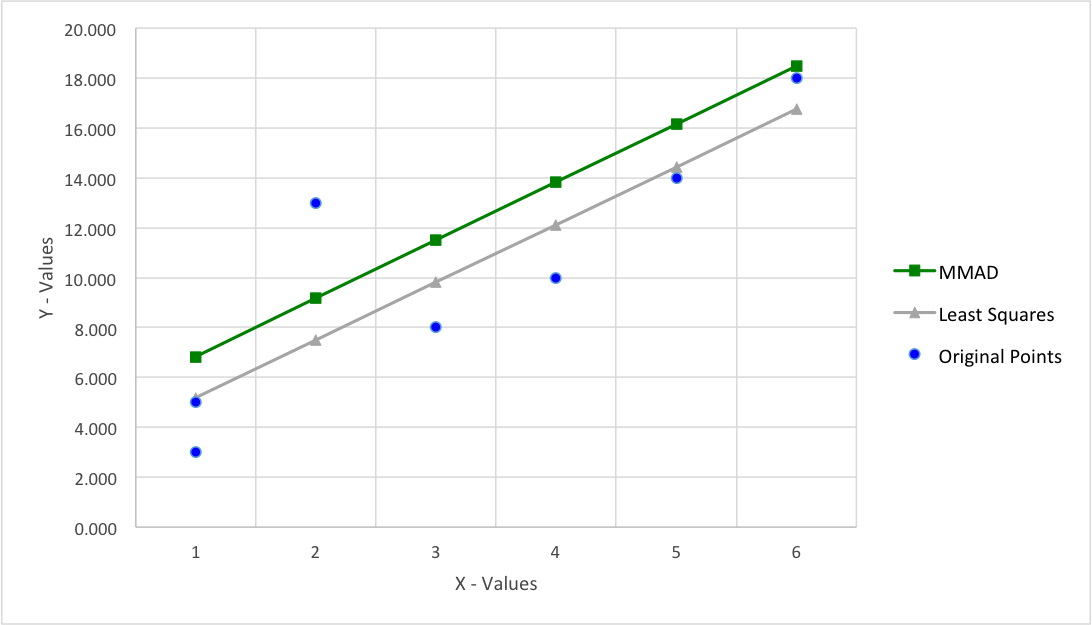
\includegraphics[width=7in]{mmad.png}}

This was calculated again in Lindo using the constraint equations above to obtain the MMAD equation $y = 2.3x + 4.5$. By contrast, the MMAD parallels the Least Squares by almost a full y-value above the Least Squares line. This makes sense since we are merely optimizing or taking the minimum of the maximum possible deviation.\vspace{8pt}

Lindo code:\vspace{8pt}

\begin{verbatim}
MIN X + Y + Z
ST
    A0+A1+Z>=3
    A0+A1-Z<=3
    A0+A1+Z>=5
    A0+A1-Z<=5
    A0+2A1+Z>=13
    A0+2A1-Z<=13
    A0+3A1+Z>=8
    A0+3A1-Z<=8
    A0+4A1+Z>=10
    A0+4A1-Z<=10
    A0+5A1+Z>=14
    A0+5A1-Z<=14
    A0+6A1+Z>=18
    A0+6A1-Z<=18
A0>0
A1>0
END
\end{verbatim}

Intuitively, it is not immediately apparent that a non-linear dataset could exist that would produce the same line using all 3 methods, but after some thought and discussion a solution presented itself. Take the following dataset:\vspace{8pt}

\hspace{20pt}(x,y) = \{ (1,2), (1, 3), (1, 4), (7, 5), (7,6), (7, 7) \}\vspace{8pt}

Testing all 3 methods in Lindo produced the same regression equation: $y = 0.5x + 2.5$. Therefore, a dataset does exist that will yield the same line via all 3 methods.


\subsection*{Part C}
\textbf{Objective}: min $\sum\limits_{i=1}^n |y_i -  (a_2x_{2i} + a_1x_{1i} + a_0)|$ as an LP.\vspace{8pt}

\textbf{Constraint Equations}

\begin{tabular}{l l l}
$a_2 + a_1 + a_0 + z_1 \geq 5$ & & $a_2 + a_1 + a_0 - z_1 \leq 5$\\
$2a_2 + a_1 + a_0 + z_2 \geq 9$ & & $2a_2 + a_1 + a_0 - z_2 \leq 9$\\
$2a_2 + 2a_1 + a_0 + z_3 \geq 12$ & & $2a_2 + 2a_1 + a_0 - z_3 \leq 12$\\
$a_2 + 0a_1 + a_0 + z_4 \geq 3$ & & $a_2 + 0a_1 + a_0 - z_4 \leq 3$\\
$0a_2 + 0a_1 + a_0 + z_5 \geq 0$ & & $0a_2 + 0a_1 + a_0 - z_5 \leq 0$\\
$3a_2 + a_1 + a_0 + z_6 \geq 11$ & & $3a_2 + a_1 + a_0 - z_6 \leq 11$\\
\end{tabular}\vspace{8pt}

This was again calculated in Lindo using the constraint equations above to obtain the LAD equation $y = 3x_2 + 3x_1$.\vspace{8pt}

\begin{verbatim}
MIN W + X + Y + Z
ST
    A0+A1+A2+Z1>=5
    A0+A1+A2-Z1<=5
    A0+A1+2A2+Z2>=9
    A0+A1+2A2-Z2<=9
    A0+2A1+2A2+Z3>=12
    A0+2A1+2A2-Z3<=12
    A0+0A1+A2+Z4>=3
    A0+0A1+A2-Z4<=3
    A0+0A1+0A2+Z5>=0
    A0+0A1+0A2-Z5<=0
    A0+A1+3A2+Z6>=11
    A0+A1+3A2-Z6<=11
A0>0
A1>0
A2>0
END
\end{verbatim}

\end{document}
